% Template adapted from https://github.com/jgm/pandoc-templates/blob/master/default.latex
% To be used with XeLaTex in memoiR
%%%%%%%%%%%%%%%%%%%%%%%%%%%%%%%%%%%%%%%%%%%%%%%%%%%%%%%%%%%%%%%%%%%%%%%%%%%%%%%%%%%%%%%%%

% Options for packages loaded elsewhere
\PassOptionsToPackage{unicode=true}{hyperref}
\PassOptionsToPackage{hyphens}{url}
\PassOptionsToPackage{dvipsnames,svgnames*,x11names*}{xcolor}
% Right to left support


\documentclass[
  10pt,
  italian,
  a4paper,
  extrafontsizes,onecolumn,openright
  ]{memoir}

% Double (or whatever) spacing

% Math
\usepackage{amssymb, amsmath}
% mathspec: arbitrary math fonts
\usepackage{unicode-math}
\defaultfontfeatures{Scale=MatchLowercase}
\defaultfontfeatures[\rmfamily]{Ligatures=TeX,Scale=1}

% Fonts
% \usepackage{lmodern}
\usepackage{fontspec}

% Main font
% Specific sanserif font
% Specific monotype font
\setmonofont[Scale=0.75]{Operator Mono SSm Book}
% Specific math font
% Chinese, Japanese, Corean fonts

% Use upquote for straight quotes in verbatim environments
\usepackage{upquote}
% Use microtype
\usepackage[]{microtype}
\UseMicrotypeSet[protrusion]{basicmath} % disable protrusion for tt fonts

% Verbatim in note

% Color links
\usepackage{xcolor}

% Strikeout

% Necessary for code chunks
\usepackage{color}
\usepackage{fancyvrb}
\newcommand{\VerbBar}{|}
\newcommand{\VERB}{\Verb[commandchars=\\\{\}]}
\DefineVerbatimEnvironment{Highlighting}{Verbatim}{commandchars=\\\{\}}
% Add ',fontsize=\small' for more characters per line
\usepackage{framed}
\definecolor{shadecolor}{RGB}{248,248,248}
\newenvironment{Shaded}{\begin{snugshade}}{\end{snugshade}}
\newcommand{\AlertTok}[1]{\textcolor[rgb]{0.94,0.16,0.16}{#1}}
\newcommand{\AnnotationTok}[1]{\textcolor[rgb]{0.56,0.35,0.01}{\textbf{\textit{#1}}}}
\newcommand{\AttributeTok}[1]{\textcolor[rgb]{0.77,0.63,0.00}{#1}}
\newcommand{\BaseNTok}[1]{\textcolor[rgb]{0.00,0.00,0.81}{#1}}
\newcommand{\BuiltInTok}[1]{#1}
\newcommand{\CharTok}[1]{\textcolor[rgb]{0.31,0.60,0.02}{#1}}
\newcommand{\CommentTok}[1]{\textcolor[rgb]{0.56,0.35,0.01}{\textit{#1}}}
\newcommand{\CommentVarTok}[1]{\textcolor[rgb]{0.56,0.35,0.01}{\textbf{\textit{#1}}}}
\newcommand{\ConstantTok}[1]{\textcolor[rgb]{0.00,0.00,0.00}{#1}}
\newcommand{\ControlFlowTok}[1]{\textcolor[rgb]{0.13,0.29,0.53}{\textbf{#1}}}
\newcommand{\DataTypeTok}[1]{\textcolor[rgb]{0.13,0.29,0.53}{#1}}
\newcommand{\DecValTok}[1]{\textcolor[rgb]{0.00,0.00,0.81}{#1}}
\newcommand{\DocumentationTok}[1]{\textcolor[rgb]{0.56,0.35,0.01}{\textbf{\textit{#1}}}}
\newcommand{\ErrorTok}[1]{\textcolor[rgb]{0.64,0.00,0.00}{\textbf{#1}}}
\newcommand{\ExtensionTok}[1]{#1}
\newcommand{\FloatTok}[1]{\textcolor[rgb]{0.00,0.00,0.81}{#1}}
\newcommand{\FunctionTok}[1]{\textcolor[rgb]{0.00,0.00,0.00}{#1}}
\newcommand{\ImportTok}[1]{#1}
\newcommand{\InformationTok}[1]{\textcolor[rgb]{0.56,0.35,0.01}{\textbf{\textit{#1}}}}
\newcommand{\KeywordTok}[1]{\textcolor[rgb]{0.13,0.29,0.53}{\textbf{#1}}}
\newcommand{\NormalTok}[1]{#1}
\newcommand{\OperatorTok}[1]{\textcolor[rgb]{0.81,0.36,0.00}{\textbf{#1}}}
\newcommand{\OtherTok}[1]{\textcolor[rgb]{0.56,0.35,0.01}{#1}}
\newcommand{\PreprocessorTok}[1]{\textcolor[rgb]{0.56,0.35,0.01}{\textit{#1}}}
\newcommand{\RegionMarkerTok}[1]{#1}
\newcommand{\SpecialCharTok}[1]{\textcolor[rgb]{0.00,0.00,0.00}{#1}}
\newcommand{\SpecialStringTok}[1]{\textcolor[rgb]{0.31,0.60,0.02}{#1}}
\newcommand{\StringTok}[1]{\textcolor[rgb]{0.31,0.60,0.02}{#1}}
\newcommand{\VariableTok}[1]{\textcolor[rgb]{0.00,0.00,0.00}{#1}}
\newcommand{\VerbatimStringTok}[1]{\textcolor[rgb]{0.31,0.60,0.02}{#1}}
\newcommand{\WarningTok}[1]{\textcolor[rgb]{0.56,0.35,0.01}{\textbf{\textit{#1}}}}

% Listings package

% Tables
\usepackage{longtable,booktabs,tabu}
% Fix footnotes in tables (requires footnote package)
\IfFileExists{footnote.sty}{\usepackage{footnote}\makesavenoteenv{longtable}}{}

% Graphics
\usepackage{graphicx,grffile}
\graphicspath{{images/}}
\makeatletter
\def\maxwidth{\ifdim\Gin@nat@width>\linewidth\linewidth\else\Gin@nat@width\fi}
\def\maxheight{\ifdim\Gin@nat@height>\textheight\textheight\else\Gin@nat@height\fi}
\makeatother
% Scale images if necessary, so that they will not overflow the page
% margins by default, and it is still possible to overwrite the defaults
% using explicit options in \includegraphics[width, height, ...]{}
\setkeys{Gin}{width=\maxwidth,height=\maxheight,keepaspectratio}

% Prevent overfull lines
\setlength{\emergencystretch}{3em}  
\providecommand{\tightlist}{%
  \setlength{\itemsep}{0pt}\setlength{\parskip}{0pt}}

% Number sections for memoir (secnumdepth counter is ignored)
\setsecnumdepth{section}

% Set default figure placement to htbp
\makeatletter
\def\fps@figure{htbp}
\makeatother

% Spacing in lists
\usepackage{enumitem}

% Polyglossia
\usepackage{polyglossia}
\setmainlanguage{it}
\setotherlanguage{en-US}

% BibLaTeX
\usepackage[backend=biber,style=authoryear-ibid,isbn=false,backref=true,giveninits=true,uniquename=init,maxcitenames=2,maxbibnames=150,sorting=nyt,sortcites=false,style=apa]{biblatex}
\addbibresource{refs.bib}
\addbibresource{packages.bib}

% cslreferences environment required by pandoc > 2.7



%%%%%%%%%%%%%%%%%%%%%%%%%%%%%%%%%%%%%%%%%%%%%%%%%%%%%%%%%%
% memoiR format

% Chapter Summary environment 
\usepackage[tikz]{bclogo}
\newenvironment{Summary}
  {\begin{bclogo}[logo=\bctrombone, noborder=true, couleur=lightgray!50]{In breve}\parindent0pt}
  {\end{bclogo}}
% Syntax:
%
%```{block, type='Summary'}
% Deliver message here.
% ```

% scriptsize code 
\let\oldverbatim\verbatim
\def\verbatim{\oldverbatim\scriptsize}
% Applies to code blocks and R code results
% code chunk options size='scriptsize' applies only to R code and results
% if the code chunk sets a different size, \def\verbatim{...} is prioritary for code results 


% Layout
%%%%%%%%%%%%%%%%%%%%%%%%%%%%%%%%%%%%%%%%%%%%%%%%%%%%%%%%%%

% Based on memoir, style companion
\newcommand{\MemoirChapStyle}{daleif1}
\newcommand{\MemoirPageStyle}{Ruled}

% Space between paragraphs
\usepackage{parskip}
  \abnormalparskip{3pt}

% Adjust margin paragraphs vertical position
\usepackage{marginfix}


% Margins
%%%%%%%%%%%%%%%%%%%%%%%%%%%%%%%%%%%%%%%

% allow use of '-',+','/' ans '*' to make simple length computation
\usepackage{calc}

% Full-width figures utilities
\newlength\widthw % full width
\newlength{\rf}
\newcommand*{\definesHSpace}{
  \strictpagecheck % slower but efficient detection of odd/even pages
  \checkoddpage
  \ifoddpage
  \setlength{\rf}{0mm}
  \else
  \setlength{\rf}{\marginparsep+\marginparwidth}
  \fi
}

\makeatletter
% 1" margins for the front matter.
\newcommand*{\SmallMargins}{
  \setlrmarginsandblock{1.5in}{1.5in}{*}
  \setmarginnotes{0.1in}{0.1in}{0.1in}
 \setulmarginsandblock{1.5in}{1in}{*}
  \checkandfixthelayout
  \ch@ngetext
  \clearpage
  \setlength{\widthw}{\textwidth+\marginparsep+\marginparwidth}
  \footnotesatfoot
  \chapterstyle{\MemoirChapStyle}  % Chapter and page styles must be recalled
  \pagestyle{\MemoirPageStyle}
}

% 3" outer margin for the main matter
\newcommand{\LargeMargins}{\SmallMargins}
\makeatother

% Figure captions and footnotes in outer margins


% Main title page with filigrane
%%%%%%%%%%%%%%%%%%%%%%%%%%%%%%%%%%%%%%%%%%%%%%%%%%%%%%%%%%

% Text blocks
\usepackage[absolute,overlay]{textpos}
  \setlength{\TPHorizModule}{1mm}
  \setlength{\TPVertModule}{1mm}

\newcommand{\MainTitlePage}[2]{
  \SmallMargins % Margins
  \pagestyle{empty} % No header/footer
  \textblockorigin{\stockwidth-\paperwidth-\trimedge}{\trimtop} % recto
  \begin{textblock*}{2mm}(\spinemargin/2,\uppermargin/2)
    \rule{1pt}{\paperheight-\uppermargin}
  \end{textblock*}
  \begin{textblock*}{\paperwidth*2/3}(\paperwidth/5, \paperheight/5)
    \flushright
    \begin{Spacing}{3}
      {\fontfamily{qtm}\selectfont\fontsize{45}{45}\selectfont\textsc{\thetitle}}
    \end{Spacing}
  \end{textblock*}
    \begin{textblock*}{\paperwidth*2/3}(\paperwidth/5, \paperheight/2)
    \flushright
    {\fontfamily{qtm}\huge\theauthor}
  \end{textblock*}
    \begin{textblock*}{\paperwidth*2/3}[0, 1](\spinemargin, \uppermargin+\textheight)
    \normalfont\thedate
  \end{textblock*}
  ~\\ % Print a character or the page will not exist
  \newpage
  \textblockorigin{\trimedge}{\trimtop} % verso
  \begin{textblock*}{\textwidth}(\paperwidth-\spinemargin-\textwidth, \uppermargin)
    #1
  \end{textblock*}
  \begin{textblock*}{\textwidth}[0,1](\paperwidth-\spinemargin-\textwidth, \uppermargin+\textheight+\footskip)
    \centering
    
\includegraphics[width=\paperwidth/4]{logo}\\ \bigskip
    #2
  \end{textblock*}
  ~\\ % Print a character or the page will not exist
  \newpage
}

% Clear page and open an even one (\clearpage opens an odd one)
\newcommand{\evenpage}{
  \clearpage
  \strictpagecheck % slower but efficient detection of odd/even pages
  \checkoddpage
  \ifoddpage
    \thispagestyle{empty}
    ~\\ % Print a character or the page will not exist
    \newpage
  \else
    % do nothing
  \fi
}


%% PDF title page to insert
%%%%%%%%%%%%%%%%%%%%%%%%%%%%%%%%%%%%%%%%%%%%%%%%%%%%%%%%%%



%% Bibliography
%%%%%%%%%%%%%%%%%%%%%%%%%%%%%%%%%%%%%%%%%%%%%%%%%%%%%%%%%%

\usepackage[strict,autostyle]{csquotes}
% Repeated citation as author-year-title instead of author-title (modification of footcite:note in verbose-inote.cbx)

%% Table of Contents
%%%%%%%%%%%%%%%%%%%%%%%%%%%%%%%%%%%%%%%%%%%%%%%%%%%%%%%%%%

% fix the typesetting of the part number
\renewcommand\partnumberlinebox[2]{#2\ ---\ }


% Fonts
%%%%%%%%%%%%%%%%%%%%%%%%%%%%%%%%%%%%%%%%%%%%%%%%%%%%%%%%%%


% Hyperref comes last
%%%%%%%%%%%%%%%%%%%%%%%%%%%%%%%%%%%%%%%%%%%%%%%%%%%%%%%%%%

\usepackage{hyperref}
\hypersetup{
  pdftitle={Psicometria},
  pdfauthor={Corrado Caudek},
  colorlinks=true,
  linkcolor=Maroon,
  citecolor=Blue,
  urlcolor=Blue,
  breaklinks=true}

% Don't use monospace font for urls
\urlstyle{same}


% Title, author, date from YAML to LaTeX
%%%%%%%%%%%%%%%%%%%%%%%%%%%%%%%%%%%%%%%%%%%%%%%%%%%%%%%%%%

\title{Psicometria}

\author{Corrado Caudek}

\date{2022-01-11}


% Include headers (preamble.tex) here
%%%%%%%%%%%%%%%%%%%%%%%%%%%%%%%%%%%%%%%%%%%%%%%%%%%%%%%%%%
% Add LaTeX code into the preamble of the document here
\hyphenation{bio-di-ver-si-ty sap-lings}


%%%%%%%%%%%%%%%%%%%%%%%%%%%%%%%%%%%%%%%%%%%%%%%%%%%%%%%%%%%%%%%%%%%%%%%%%
% memoiR dalef3 chapter style 
% https://ctan.crest.fr/tex-archive/info/latex-samples/MemoirChapStyles/MemoirChapStyles.pdf
\usepackage{amsmath}

\usepackage{soul}
\definecolor{nicered}{rgb}{.647,.129,.149}

\makeatletter
\makechapterstyle{pedersen}
\makeatother

\DeclareMathOperator{\Var}{Var} % Define variance operator
\DeclareMathOperator{\SD}{SD} % Define sd operator
\DeclareMathOperator{\Cov}{Cov} % Define covariance operator
\DeclareMathOperator{\Corr}{Corr} % Define correlation operator
\DeclareMathOperator{\Me}{Me} % Define mediane operator
\DeclareMathOperator{\Mo}{Mo} % Define mode operator
\DeclareMathOperator{\Bin}{Bin} % Define binomial operator
\DeclareMathOperator{\Bernoulli}{Bernoulli} % Define Bernoulli operator
\DeclareMathOperator{\Poi}{Poi} % Define Poisson operator
\DeclareMathOperator{\Uniform}{Uniform} % Define Uniform operator
\DeclareMathOperator{\Cauchy}{Cauchy} % Define Cauchy operator
\DeclareMathOperator{\elpd}{elpd} % Define elpd operator
\DeclareMathOperator{\lppd}{lppd} % Define lppd operator
\DeclareMathOperator{\LOO}{LOO} % Define LOO operator
\DeclareMathOperator{\Ber}{\mathscr{B}} % Define Bernoulli operator
\DeclareMathOperator{\B}{B} % beta function
% \mbox{B}(a, b) % beta function
% \mbox{Beta}(a, b) % beta distribution
\newcommand{\R}{\textsf{R}} % Define R programming language symbol
\newcommand{\E}{\mathbb{E}} % Define expected value operator
\newcommand{\Real}{\mathbb{R}} % Define real number operator
\newcommand{\Prob}{\mathscr{P}}
\DeclareMathOperator{\argmin}{arg\,min} % thin space, limits on side in displays
\DeclareMathOperator{\argmax}{arg\,max} % no space, limits on side in displays

\raggedbottom % allow variable (ragged) site heights
\frenchspacing

\usepackage[
  labelfont=bf, 
  font={small, it} 
]{caption} 
\usepackage{upquote} % print correct quotes in verbatim-environments
\usepackage{empheq} 
\usepackage{xfrac}
%\usepackage{lstbayes}
%\usepackage{awesomebox}



\usepackage{booktabs}
\usepackage{longtable}
\usepackage{array}
\usepackage{multirow}
\usepackage{wrapfig}
\usepackage{float}
\usepackage{colortbl}
\usepackage{pdflscape}
\usepackage{tabu}
\usepackage{threeparttable}
\usepackage{threeparttablex}
\usepackage[normalem]{ulem}
\usepackage{makecell}
\usepackage{xcolor}


% End of preamble
%%%%%%%%%%%%%%%%%%%%%%%%%%%%%%%%%%%%%%%%%%%%%%%%%%%%%%%%%%


\usepackage{amsthm}
\newtheorem{theorem}{Teorema}[chapter]
\newtheorem{lemma}{Lemma}[chapter]
\newtheorem{corollary}{Corollario}[chapter]
\newtheorem{proposition}{Proposizione}[chapter]
\newtheorem{conjecture}{Congettura}[chapter]
\theoremstyle{definition}
\newtheorem{definition}{Definizione}[chapter]
\theoremstyle{definition}
\newtheorem{example}{Esempio}[chapter]
\theoremstyle{definition}
\newtheorem{exercise}{Esercizio}[chapter]
\theoremstyle{definition}
\newtheorem{hypothesis}{Hypothesis}[chapter]
\theoremstyle{remark}
\newtheorem*{remark}{Osservazione}
\newtheorem*{solution}{Soluzione}
\begin{document}
\frontmatter

% Title page
%%%%%%%%%%%%%%%%%%%%%%%%%%%%%%%%%%%%%%%%%%%%%%%%%%%%%%%%%%


\MainTitlePage{Questo documento è stato realizzato con:

\begin{itemize}
  \item \LaTeX\; e la classe memoir (\url{http://www.ctan.org/pkg/memoir});
  \item $\R$ (\url{http://www.r-project.org/}) e RStudio (\url{http://www.rstudio.com/});
  \item bookdown (\url{http://bookdown.org/}) e memoiR (\url{https://ericmarcon.github.io/memoiR/}).
  \end{itemize}}{Nel blog della mia pagina personale sono forniti alcuni approfondimenti degli argomenti qui trattati.
\url{https://ccaudek.github.io/caudeklab/}}


% Before Body
%%%%%%%%%%%%%%%%%%%%%%%%%%%%%%%%%%%%%%%%%%%%%%%%%%%%%%%%%%





% Contents
%%%%%%%%%%%%%%%%%%%%%%%%%%%%%%%%%%%%%%%%%%%%%%%%%%%%%%%%%%

\LargeMargins
{
\hypersetup{linkcolor=}
\setcounter{tocdepth}{3}
\tableofcontents
}


% Body
%%%%%%%%%%%%%%%%%%%%%%%%%%%%%%%%%%%%%%%%%%%%%%%%%%%%%%%%%%

\LargeMargins
\scriptsize

\normalsize

\chapter*{}

\vfill

\scriptsize

\normalsize

Data della versione presente: Gennaio 11, 2022.

\hypertarget{prefazione}{%
\chapter{Prefazione}\label{prefazione}}

\emph{Data Science per psicologi} contiene il materiale delle lezioni dell'insegnamento di \emph{Psicometria B000286} (A.A. 2021/2022) rivolto agli studenti del primo anno del Corso di Laurea in Scienze e Tecniche Psicologiche dell'Università degli Studi di Firenze. \emph{Psicometria} si propone di fornire agli studenti un'introduzione all'analisi dei dati in psicologia. Le conoscenze/competenze che verranno sviluppate in questo insegnamento sono quelle della Data science, ovvero un insieme di conoscenze/competenze che si pongono all'intersezione tra statistica (ovvero, richiedono la capacità di comprendere teoremi statistici) e informatica (ovvero, richiedono la capacità di sapere utilizzare un software).

\hypertarget{la-psicologia-e-la-data-science}{%
\section{La psicologia e la Data science}\label{la-psicologia-e-la-data-science}}

\begin{quote}
\emph{It's worth noting, before getting started, that this material is hard. If you find yourself confused at any point, you are normal. Any sense of confusion you feel is just your brain correctly calibrating to the subject matter. Over time, confusion is replaced by comprehension {[}\ldots{]}}

\hfill --- Richard McElreath
\end{quote}

Sembra sensato spendere due parole su un tema che è importante per gli studenti: quello indicato dal titolo di questo Capitolo. È ovvio che agli studenti di psicologia la statistica non piace. Se piacesse, forse studierebbero Data science e non psicologia; ma non lo fanno. Di conseguenza, gli studenti di psicologia si chiedono: ``perché dobbiamo perdere tanto tempo a studiare queste cose quando in realtà quello che ci interessa è tutt'altro?'' Questa è una bella domanda.

C'è una ragione molto semplice che dovrebbe farci capire perché la Data science è così importante per la psicologia. Infatti, a ben pensarci, la psicologia è una disciplina intrinsecamente statistica, se per statistica intendiamo quella disciplina che studia la variazione delle caratteristiche degli individui nella popolazione. La psicologia studia \emph{gli individui} ed è proprio la variabilità inter- e intra-individuale ciò che vogliamo descrivere e, in certi casi, predire. In questo senso, la psicologia è molto diversa dall'ingegneria, per esempio. Le proprietà di un determinato ponte sotto certe condizioni, ad esempio, sono molto simili a quelle di un altro ponte, sotto le medesime condizioni. Quindi, per un ingegnere la statistica è poco importante: le proprietà dei materiali sono unicamente dipendenti dalla loro composizione e restano costanti. Ma lo stesso non può dirsi degli individui: ogni individuo è unico e cambia nel tempo. E le variazioni tra gli individui, e di un individuo nel tempo, sono l'oggetto di studio proprio della psicologia: è dunque chiaro che i problemi che la psicologia si pone sono molto diversi da quelli affrontati, per esempio, dagli ingegneri. Questa è la ragione per cui abbiamo tanto bisogno della Data science in psicologia: perché la Data science ci consente di descrivere la variazione e il cambiamento. E queste sono appunto le caratteristiche di base dei fenomeni psicologici.

Sono sicuro che, leggendo queste righe, a molti studenti sarà venuta in mente la seguente domanda: perché non chiediamo a qualche esperto di fare il ``lavoro sporco'' (ovvero le analisi statistiche) per noi, mentre noi (gli psicologi) ci occupiamo solo di ciò che ci interessa, ovvero dei problemi psicologici slegati dai dettagli ``tecnici'' della Data science? La risposta a questa domanda è che non è possibile progettare uno studio psicologico sensato senza avere almeno una comprensione rudimentale della Data science. Le tematiche della Data science non possono essere ignorate né dai ricercatori in psicologia né da coloro che svolgono la professione di psicologo al di fuori dell'Università. Infatti, anche i professionisti al di fuori dall'università non possono fare a meno di leggere la letteratura psicologica più recente: il continuo aggiornamento delle conoscenze è infatti richiesto dalla deontologia della professione. Ma per potere fare questo è necessario conoscere un bel po' di Data science! Basta aprire a caso una rivista specialistica di psicologia per rendersi conto di quanto ciò sia vero: gli articoli che riportano i risultati delle ricerche psicologiche sono zeppi di analisi statistiche e di modelli formali. E la comprensione della letteratura psicologica rappresenta un requisito minimo nel bagaglio professionale dello psicologo.

Le considerazioni precedenti cercano di chiarire il seguente punto: la Data science non è qualcosa da studiare a malincuore, in un singolo insegnamento universitario, per poi poterla tranquillamente dimenticare. Nel bene e nel male, gli psicologi usano gli strumenti della Data science in tantissimi ambiti della loro attività professionale: in particolare quando costruiscono, somministrano e interpretano i test psicometrici. È dunque chiaro che possedere delle solide basi di Data science è un tassello imprescindibile del bagaglio professionale dello psicologo. In questo insegnamento verrano trattati i temi base della Data science e verrà adottato un punto di vista bayesiano, che corrisponde all'approccio più recente e sempre più diffuso in psicologia.

\hypertarget{come-studiare}{%
\section{Come studiare}\label{come-studiare}}

\begin{quote}
\emph{I know quite certainly that I myself have no special talent. Curiosity, obsession and dogged endurance, combined with self-criticism, have brought me to my ideas.}

\hfill --- Albert Einstein
\end{quote}

Il giusto metodo di studio per prepararsi all'esame di Psicometria è quello di seguire attivamente le lezioni, assimilare i concetti via via che essi vengono presentati e verificare in autonomia le procedure presentate a lezione. Incoraggio gli studenti a farmi domande per chiarire ciò che non è stato capito appieno. Incoraggio gli studenti a utilizzare i forum attivi su Moodle e, soprattutto, a svolgere gli esercizi proposti su Moodle. I problemi forniti su Moodle rappresentano il livello di difficoltà richiesto per superare l'esame e consentono allo studente di comprendere se le competenze sviluppate fino a quel punto sono sufficienti rispetto alle richieste dell'esame.

La prima fase dello studio, che è sicuramente individuale, è quella in cui è necessario acquisire le conoscenze teoriche relative ai problemi che saranno presentati all'esame. La seconda fase di studio, che può essere facilitata da scambi con altri e da incontri di gruppo, porta ad acquisire la capacità di applicare le conoscenze: è necessario capire come usare un software (\(\textsf{R}\)) per applicare i concetti statistici alla specifica situazione del problema che si vuole risolvere. Le due fasi non sono però separate: il saper fare molto spesso ci aiuta a capire meglio.

\hypertarget{sviluppare-un-metodo-di-studio-efficace}{%
\section*{Sviluppare un metodo di studio efficace}\label{sviluppare-un-metodo-di-studio-efficace}}
\addcontentsline{toc}{section}{Sviluppare un metodo di studio efficace}

\begin{quote}
\emph{Memorization is not learning.}

\hfill --- Richard Phillips Feynman
\end{quote}

Avendo insegnato molte volte in passato un corso introduttivo di analisi dei dati ho notato nel corso degli anni che gli studenti con l'atteggiamento mentale che descriverò qui sotto generalmente ottengono ottimi risultati. Alcuni studenti sviluppano naturalmente questo approccio allo studio, ma altri hanno bisogno di fare uno sforzo per maturarlo. Fornisco qui sotto una breve descrizione del ``metodo di studio'' che, nella mia esperienza, è il più efficace per affrontare le richieste di questo insegnamento \autocite{burger20125}.

\begin{itemize}
\tightlist
\item
  Dedicate un tempo sufficiente al materiale di base, apparentemente facile; assicuratevi di averlo capito bene. Cercate le lacune nella vostra comprensione. Leggere presentazioni diverse dello stesso materiale (in libri o articoli diversi) può fornire nuove intuizioni.
\item
  Gli errori che facciamo sono i nostri migliori maestri. Istintivamente cerchiamo di dimenticare subito i nostri errori. Ma il miglior modo di imparare è apprendere dagli errori che commettiamo. In questo senso, una soluzione corretta è meno utile di una soluzione sbagliata. Quando commettiamo un errore questo ci fornisce un'informazione importante: ci fa capire qual è il materiale di studio sul quale dobbiamo ritornare e che dobbiamo capire meglio.
\item
  C'è ovviamente un aspetto ``psicologico'' nello studio. Quando un esercizio o problema ci sembra incomprensibile, la cosa migliore da fare è dire: ``mi arrendo'', ``non ho idea di cosa fare!''. Questo ci rilassa: ci siamo già arresi, quindi non abbiamo niente da perdere, non dobbiamo più preoccuparci. Ma non dobbiamo fermarci qui. Le cose ``migliori'' che faccio (se ci sono) le faccio quando non ho voglia di lavorare. Alle volte, quando c'è qualcosa che non so fare e non ho idea di come affontare, mi dico: ``oggi non ho proprio voglia di fare fatica'', non ho voglia di mettermi nello stato mentale per cui ``in 10 minuti devo risolvere il problema perché dopo devo fare altre cose''. Però ho voglia di \emph{divertirmi} con quel problema e allora mi dedico a qualche aspetto ``marginale'' del problema, che so come affrontare, oppure considero l'aspetto più difficile del problema, quello che non so come risolvere, ma invece di cercare di risolverlo, guardo come altre persone hanno affrontato problemi simili, opppure lo stesso problema in un altro contesto. Non mi pongo l'obiettivo ``risolvi il problema in 10 minuti'', ma invece quello di farmi un'idea ``generale'' del problema, o quello di capire un caso più specifico e più semplice del problema. Senza nessuna pressione. Infatti, in quel momento ho deciso di non lavorare (ovvero, di non fare fatica). Va benissimo se ``parto per la tangente'', ovvero se mi metto a leggere del materiale che sembra avere poco a che fare con il problema centrale (le nostre intuizioni e la nostra curiosità solitamente ci indirizzano sulla strada giusta). Quando faccio così, molto spesso trovo la soluzione del problema che mi ero posto e, paradossalmente, la trovo in un tempo minore di quello che, in precedenza, avevo dedicato a ``lavorare'' al problema. Allora perché non faccio sempre così? C'è ovviamente l'aspetto dei ``10 minuti'' che non è sempre facile da dimenticare. Sotto pressione, possiamo solo agire in maniera automatica, ovvero possiamo solo applicare qualcosa che già sappiamo fare. Ma se dobbiamo imparare qualcosa di nuovo, la pressione è un impedimento.
\item
  È utile farsi da soli delle domande sugli argomenti trattati, senza limitarsi a cercare di risolvere gli esercizi che vengono assegnati. Quando studio qualcosa mi viene in mente: ``se questo è vero, allora deve succedere quest'altra cosa''. Allora verifico se questo è vero, di solito con una simulazione. Se i risultati della simulazione sono quelli che mi aspetto, allora vuol dire che ho capito. Se i risultati sono diversi da quelli che mi aspettavo, allora mi rendo conto di non avere capito e ritorno indietro a studiare con più attenzione la teoria che pensavo di avere capito -- e ovviamente mi rendo conto che c'era un aspetto che avevo frainteso. Questo tipo di verifica è qualcosa che dobbiamo fare da soli, in prima persona: nessun altro può fare questo al posto nostro.
\item
  Non aspettatevi di capire tutto la prima volta che incontrate un argomento nuovo.\footnote{Ricordatevi inoltre che gli individui tendono a sottostimare la propria capacità di apprendere \autocite{horn2021underestimating}.} È utile farsi una nota mentalmente delle lacune nella vostra comprensione e tornare su di esse in seguito per carcare di colmarle. L'atteggiamento naturale, quando non capiamo i dettagli di qualcosa, è quello di pensare: ``non importa, ho capito in maniera approssimativa questo punto, non devo preoccuparmi del resto''. Ma in realtà non è vero: se la nostra comprensione è superficiale, quando il problema verrà presentato in una nuova forma, non riusciremo a risolverlo. Per cui i dubbi che ci vengono quando studiamo qualcosa sono il nostro alleato più prezioso: ci dicono esattamente quali sono gli aspetti che dobbiamo approfondire per potere migliorare la nostra preparazione.
\item
  È utile sviluppare una visione d'insieme degli argomenti trattati, capire l'obiettivo generale che si vuole raggiungere e avere chiaro il contributo che i vari pezzi di informazione forniscono al raggiungimento di tale obiettivo. Questa organizzazione mentale del materiale di studio facilita la comprensione. È estremamente utile creare degli schemi di ciò che si sta studiando. Non aspettate che sia io a fornirvi un riepilogo di ciò che dovete imparare: sviluppate da soli tali schemi e tali riassunti.
\item
  Tutti noi dobbiamo imparare l'arte di trovare le informazioni, non solo nel caso di questo insegnamento. Quando vi trovate di fronte a qualcosa che non capite, o ottenete un oscuro messaggio di errore da un software, ricordatevi: ``Google is your friend''.
\end{itemize}

\bigskip

Corrado Caudek

\mainmatter

\hypertarget{part-inferenza-statistica-bayesiana}{%
\part*{Inferenza statistica bayesiana}\label{part-inferenza-statistica-bayesiana}}
\addcontentsline{toc}{part}{Inferenza statistica bayesiana}

\hypertarget{chapter-intro-bayes-inference}{%
\chapter{I modelli bayesiani}\label{chapter-intro-bayes-inference}}

I modelli bayesiani, computazionali o meno, hanno due caratteristiche distintive:

\begin{itemize}
\tightlist
\item
  Le quantità incognite sono descritte utilizzando le distribuzioni di probabilità. Queste quantità incognite sono chiatame parametri.
\item
  Il teorema di Bayes viene utilizzato per aggiornare i valori dei parametri condizionati ai
  dati. Possiamo anche concepire questo processo come una riallocazione delle probabilità.
\end{itemize}

\begin{remark}
Un modello è uno strumento concettuale che viene utilizzato per risolvere uno specifico problema. In quanto tale, è generalmente più conveniente parlare dell'adeguatezza del modello a un dato problema che di determinare la sua intrinseca correttezza. I modelli esistono esclusivamente come l'ausilio per il raggiungimento di un qualche ulteriore obiettivo. Il problema che i modelli bayesiani cercano di risolvere è quello dell'inferenza\footnote{In termini colloquiali, l'inferenza può essere descritta come la capacità di giungere a conclusioni basate su evidenze e ragionamenti. L'inferenza bayesiana è una particolare forma di inferenza statistica basata sulla combinazione di distribuzioni di probabilità che ha il fine di ottenere altre distribuzioni di probabilità. Nello specifico, la regola di Bayes ci fornisce un metodo per giungere alla quantificazione della plausibilità di una teoria alla luce dei dati osservati.}.
\end{remark}

Seguendo \autocite{martin2022bayesian}, possiamo descrivere il processo di costruzione della modellazione bayesiana distinguendo 3 passaggi.

\begin{enumerate}
\def\labelenumi{\arabic{enumi}.}
\tightlist
\item
  Dati alcuni dati e alcune ipotesi su come questi dati potrebbero essere stati generati, progettiamo un modello combinando e trasformando variabili casuali.
\item
  Usiamo il teorema di Bayes per condizionare i nostri modelli ai dati disponibili. Chiamiamo questo processo ``inferenza'' e come risultato otteniamo una distribuzione a posteriori. Ci auguriamo che i dati riducano l'incertezza per i possibili valori dei parametri, sebbene questo non sia garantito per nessun modello bayesiano.
\item
  Critichiamo il modello verificando se il modello abbia senso utilizzando criteri diversi, inclusi i dati e la nostra conoscenza del dominio. Poiché generalmente siamo incerti sui modelli stessi, a volte confrontiamo diversi modelli.
\end{enumerate}

Questi 3 passaggi vengono eseguiti in modo iterativo e danno luogo a quello che si chiama un ``flusso di lavoro bayesiano'' (\emph{bayesian workflow}).

\hypertarget{il-problema-inverso}{%
\section{Il problema inverso}\label{il-problema-inverso}}

In questo capitolo ci focalizzeremo sul passaggio 2 descritto sopra. Nello specifico, descrivemo in dettaglio il significato dei tre i termini a destra del segno di uguale nella formula di Bayes: la distribuzione a priori e la funzione di verosimiglianza al numeratore, e la verosimiglianza marginale al denominatore.

\begin{remark}
La moderna statistica bayesiana viene per lo più eseguita utilizzando un linguaggio di programmazione probabilistico implementato su computer. Ciò ha cambiato radicalmente il modo in cui venivano eseguite le statistiche bayesiane anche fin pochi decenni fa. La complessità dei modelli che possiamo costruire è aumentata e la barriera delle competenze matematiche e computazionali che sono richieste è diminuita. Inoltre, il processo di modellazione iterativa è diventato, sotto molti aspetti, molto più facile da eseguire. Anche se formulare modelli statistici complessi è diventato più facile che mai, la statistica è un campo pieno di sottigliezze che non scompaiono magicamente utilizzando potenti metodi computazionali. Pertanto, avere una buona preparazione sugli aspetti teorici, specialmente quelli rilevanti nella pratica, è estremamente utile per applicare efficacemente i metodi statistici.
\end{remark}

\hypertarget{inferenza-bayesiana-come-un-problema-inverso}{%
\section{Inferenza bayesiana come un problema inverso}\label{inferenza-bayesiana-come-un-problema-inverso}}

\hypertarget{notazione}{%
\subsection{Notazione}\label{notazione}}

Per fissare la notazione, nel seguito \(y\) rappresenterà i dati e \(\theta\) rappresenterà i parametri incogniti di un modello statistico. Sia \(y\) che \(\theta\) saranno concepiti come delle variabili casuali.\footnote{Nell'approccio bayesiano si fa riferimento ad un modello probabilistico \(f(y \mid \theta)\) rappresentativo del fenomeno d'interesse noto a meno del valore assunto dal parametro (o dei parametri) che lo caratterizza. Si fa inoltre riferimento ad una distribuzione congiunta (di massa o di densità di probabilità) \(f(y, \theta)\). Entrambi gli argomenti della funzione \(y\) e \(\theta\) hanno natura di variabili casuali, laddove la nostra incertezza relativa a \(y\) è dovuta alla naturale variabilità del fenomeno indagato (\emph{variabilità aleatoria}), mentre la nostra incertezza relativa a \(\theta\) è dovuta alla mancata conoscenza del suo valore numerico (\emph{variabilità epistemica}).} Con \(x\) verranno invece denotate le quantità note, come ad esempio i predittori del modello lineare. Per rappresentare in un modo conciso i modelli probabilistici viene usata una notazione particolare. Ad esempio, invece di scrivere \(p(\theta) = \mbox{Beta}(1, 1)\)
scriviamo \(\theta \sim \mbox{Beta}(1, 1)\). Il simbolo ``\(\sim\)'' viene spesso letto ``è distribuito come''. Possiamo anche pensare che significhi che \(\theta\) costituisce un campione casuale estratto dalla distribuzione Beta(1, 1). Allo stesso modo, ad esempio, la verosimiglianza del modello binomiale può essere scritta come \(y \sim \text{Bin}(n, \theta)\).

\hypertarget{funzioni-di-probabilituxe0}{%
\subsection{Funzioni di probabilità}\label{funzioni-di-probabilituxe0}}

Una caratteristica attraente della statistica bayesiana è che la nostra credenza ``a posteriori'' viene sempre descritta mediante una distribuzione. Questo fatto ci consente di fare affermazioni probabilistiche sui parametri, come ad esempio: ``la probabilità che un parametro sia positivo è 0.35''; oppure, ``il valore più probabile di \(\theta\) è 12 e abbiamo probabilità del 50\% che \(\theta\) sia compreso tra 10 e 15''. Inoltre, possiamo pensare alla distribuzione a posteriori come alla logica conseguenza della combinazione di un modello con i dati; quindi, abbiamo la garanzia che le affermazioni probabilistiche associate alla distribuzione a posteriori siano matematicamente coerenti. Dobbiamo solo ricordare che tutte queste belle proprietà matematiche sono valide solo nel mondo platonico delle idee dove esistono oggetti matematici come sfere, distribuzioni gaussiane e catene di Markov. Quando passiamo dalla purezza della matematica al disordine della matematica applicata al mondo reale, dobbiamo sempre tenere a mente che i nostri risultati sono condizionati, non solo dai dati, ma anche dai modelli. Di conseguenza, dati errati e/o modelli errati conducono facilmente a conclusioni prive di senso, anche se matematicamente coerenti. È dunque necessario conservare sempre una sana quota di scetticismo relativamente ai nostri dati, modelli e risultati \autocite{martin2022bayesian}.

Avendo detto questo, nell'aggiornamento bayesiano (dai dati ai parametri) vengono utilizzate le seguenti distribuzioni di probabilità (o di massa di probabilità):

\begin{itemize}
\tightlist
\item
  la \emph{distribuzione a priori} \(p(\theta)\) --- la credenza iniziale (prima di avere osservato i dati \(Y = y\)) riguardo a \(\theta\);
\item
  la \emph{funzione di verosimiglianza} \(p(y \mid \theta)\) --- quanto sono compatibili i dati osservati \(Y = y\) con i diversi valori possibili di \(\theta\)?
\item
  la \emph{verosimiglianza marginale} \(p(y)\) --- costante di normalizzazione: qual è la probabilità complessiva di osservare i dati \(Y = y\)? In termini formali:
  \[
  p(y) = \int_\theta p(y, \theta) \,\operatorname {d}\!\theta = \int_\theta p(y \mid \theta) p(\theta) \,\operatorname {d}\!\theta.
  \]
\item
  la \emph{distribuzione a posteriori} \(p(\theta \mid y)\) --- la nuova credenza relativa alla credibilità di ciascun valore \(\theta\) dopo avere osservato i dati \(Y = y\).
\end{itemize}

\hypertarget{la-regola-di-bayes}{%
\section{La regola di Bayes}\label{la-regola-di-bayes}}

Assumendo un modello statistico, la formula di Bayes consente di giungere alla distribuzione a posteriori \(p(\theta \mid y)\) per il parametro di interesse \(\theta\), come indicato dalla seguente catena di equazioni\footnote{In realtà, avremmo dovuto scrivere \(p(\theta \mid y, \mathcal{M})\), in quanto non condizioniamo la stima di \(\theta\) solo rispetto ai dati \(y\) ma anche ad un modello probabilistico \(\mathcal{M}\) che viene assunto quale meccanismo generatore dei dati. Per semplicità di notazione, omettiamo il riferimento a \(\mathcal{M}\).}:
\begin{align}
p(\theta \mid y)  &= \displaystyle \frac{p(\theta,y)}{p(y)}
 \ \ \ \ \ \mbox{ [definizione di probabilità condizionata]}
\\
&= \displaystyle \frac{p(y \mid \theta) \, p(\theta)}{p(y)}
 \ \ \ \ \ \mbox{ [legge della probabilità composta]}
\\
&=  \displaystyle \frac{p(y \mid\theta) \, p(\theta)}
                        {\int_{\Theta} p(y,\theta) \, \,\operatorname {d}\!\theta}
 \ \ \ \ \ \mbox{ [legge della probabilità totale]}
\\
&= \displaystyle \frac{p(y \mid\theta) \, p(\theta)}
                        {\int_{\Theta} p(y \mid\theta) \, p(\theta) \, \,\operatorname {d}\!\theta}
 \ \ \ \ \ \mbox{ [legge della probabilità composta]}
\\
& \propto \displaystyle p(y \mid\theta) \, p(\theta)
\label{eq:bayesmodel}
\end{align}

La regola di Bayes ``inverte'' la probabilità della distribuzione a posteriori \(p(\theta \mid y)\), esprimendola nei termini della funzione di verosimiglianza \(p(y \mid \theta)\) e della distribuzione a priori \(p(\theta)\). L'ultimo passo è importante per la stima della distribuzione a posteriori mediante i metodi Monte Carlo a catena di Markov, in quanto per questi metodi richiedono soltanto che le funzioni di probabilità siano definite a meno di una costante di proporzionalità. In altri termini, per la maggior parte degli scopi dell'inferenza inversa, è sufficiente calcolare la densità a posteriori non normalizzata, ovvero è possibile ignorare il denominatore bayesiano \(p(y)\). La distribuzione a posteriori non normalizzata, dunque, si riduce al prodotto della varosimiglianza e della distribuzione a priori.

Possiamo dire che la regola di Bayes viene usata per aggiornare le credenze a priori su \(\theta\) (ovvero, la distribuzione a priori) in modo tale da produrre le nuove credenze a posteriori \(p(\theta \mid y)\) che combinano le informazioni fornite dai dati \(y\) con le credenze precedenti. La distribuzione a posteriori riflette dunque l'aggiornamento delle credenze del ricercatore alla luce dei dati. La distribuzione a posteriori \(p(\theta \mid y)\) contiene tutta l'informazione riguardante il parametro \(\theta\) e viene utilizzata per produrre indicatori sintetici, per la determinazione di stime puntuali o intervallari, e per la verifica d'ipotesi.

La \eqref{eq:bayesmodel} rende evidente che, in ottica bayesiana, la quantità di interesse \(\theta\) non è fissata (come nell'impostazione frequentista), ma è una variabile casuale la cui distribuzione di probabilità è influenzata sia dalle informazioni a priori sia dai dati a disposizione. In altre parole, nell'approccio bayesiano non esiste un valore vero di \(\theta\), ma invece lo scopo è quello di fornire invece un giudizio di probabilità (o di formulare una ``previsione'', nel linguaggio di de Finetti). Prima delle osservazioni, sulla base delle nostre conoscenze assegnamo a \(\theta\) una distribuzione a priori di probabilità. Dopo le osservazioni, correggiamo il nostro giudizio e assegniamo a \(\theta\) una distribuzione a posteriori di probabilità.

\hypertarget{un-esempio-di-aggiornamento-bayesiano}{%
\subsection{Un esempio di aggiornamento bayesiano}\label{un-esempio-di-aggiornamento-bayesiano}}

Per descrivere l'aggiornamento bayesiano, in questo Capitolo (così come nei successivi) considereremo i dati di \textcite{zetschefuture2019}. Questi ricercatori si sono chiesti se gli individui depressi manifestino delle aspettative accurate circa il loro umore futuro, oppure se tali aspettative siano distorte negativamente. Esamineremo qui i 30 partecipanti dello studio di \textcite{zetschefuture2019} che hanno riportato la presenza di un episodio di depressione maggiore in atto. All'inizio della settimana di test, a questi pazienti è stato chiesto di valutare l'umore che si aspettavano di esperire nei giorni seguenti della settimana. Mediante una app, i partecipanti dovevano poi valutare il proprio umore in cinque momenti diversi di ciascuno dei cinque giorni successivi. Lo studio considera diverse emozioni, ma qui ci concentriamo solo sulla tristezza.

Sulla base dei dati forniti dagli autori, abbiamo calcolato la media dei giudizi relativi al livello di tristezza raccolti da ciascun partecipante tramite la app. Tale media è stata poi sottratta dall'aspettativa del livello di tristezza fornita all'inizio della settimana. La discrepanza tra aspettative e realtà è stata considerata come un evento dicotomico: valori positivi di tale differenza indicano che le aspettative circa il livello di tristezza erano maggiori del livello di tristezza effettivamente esperito --- ciò significa che le aspettative future risultano negativamente distorte (evento codificato con ``1''). Viceversa, si ha che le aspettative risultano positivamente distorte se la differenza descritta in precedenza assume un valore negativo (evento codificato con ``0'').

Nel campione dei 30 partecipanti clinici di \textcite{zetschefuture2019}, le aspettative future di 23 partecipanti risultano distorte negativamente e quelle di 7 partecipanti risultano distorte positivamente. Chiameremo \(\theta\) la probabilità dell'evento ``le aspettative del partecipante sono distorte negativamente''. Ci poniamo il problema di ottenere una stima a posteriori di \(\theta\) avendo osservato 23 ``successi'' in 30 prove.\footnote{Si noti un punto importante: dire semplicemente che la stima di \(\theta\) è uguale a 23/30 = 0.77 ci porta ad ignorare il livello di incertezza associato a tale stima. Infatti, lo stesso valore (0.77) si può ottenere come 23/30, o 230/300, o 2300/3000, o 23000/30000, ma l'incertezza di una stima pari a 0.77 è molto diversa nei quattro casi. Quando si traggono conclusioni dai dati è invece necessario quantificare il livello della nostra incertezza relativamente alla stima del parametro di interesse (nel caso presente, \(\theta\)). Lo strumento ci consente di quantificare tale incertezza è la distribizione a posteriori \(p(\theta \mid y)\). Ovviamente, \(p(\theta \mid y)\) assume forme molto diverse nei quattro casi descritti sopra.}

\hypertarget{modello-probabilistico}{%
\section{Modello probabilistico}\label{modello-probabilistico}}

Nel caso dello studio di \textcite{zetschefuture2019}, i dati qui considerati possono essere considerati la manifestazione di una variabile casuale Bernoulliana -- 23 ``successi'' in 30 prove. Se i dati rappresentano una proporzione, allora possiamo adottare un modello probabilistico binomiale quale meccanismo generatore dei dati:
\begin{equation}
y  \sim \mbox{Bin}(n, \theta),
\label{eq:binomialmodel}
\end{equation}
laddove \(\theta\) è la probabiltà che una prova Bernoulliana assuma il valore 1 e \(n\) corrisponde al numero di prove Bernoulliane. Questo modello assume che le prove Bernoulliane \(y_i\) che costituiscono il campione \(y\) siano tra loro indipendenti e che ciascuna abbia la stessa probabilità \(\theta \in [0, 1]\) di essere un ``successo'' (valore 1). In altre parole, il modello generatore dei dati avrà una funzione di massa di probabilità
\[
p(y \mid \theta)
\ = \
\mbox{Bin}(y \mid n, \theta).
\]

Nei capitoli precedenti è stato mostrato come, sulla base del modello binomiale, sia possibile assegnare una probabilità a ciascun possibile valore \(y \in \{0, 1, \dots, n\}\) \emph{assumendo noto il valore del parametro} \(\theta\). Ma ora abbiamo il problema inverso, ovvero quello di fare inferenza su \(\theta\) alla luce dei dati campionari \(y\). In altre parole, riteniamo di conoscere il modello probabilistico che ha generato i dati, ma di tale modello non conosciamo i parametri: vogliamo dunque ottenere informazioni su \(\theta\) avendo osservato i dati \(y\).

Nel modello probabilistico che stiamo esaminando, il termine \(n\) viene trattato come una costante nota e \(\theta\) come una \emph{variabile casuale}.
Dato che \(\theta\) è incognito, ma abbiamo a disposione i dati \(y\), svolgeremo l'inferenza su \(\theta\) mediante la regola di Bayes per determinare la distribuzione a posteriori \(p(\theta \mid y)\).

\begin{remark}
Si noti che il modello probabilistico \eqref{eq:binomialmodel} non spiega perché, in ciascuna realizzazione, \(Y\) assuma un particolare valore. Questo modello deve piuttosto essere inteso come un costrutto matematico che ha lo scopo di riflettere alcune proprietà del processo corrispondente ad una sequenza di prove Bernoulliane. Una parte del lavoro della ricerca in tutte le scienze consiste nel verificare le assunzioni dei modelli e, se necessario, nel migliorare i modelli dei fenomeni considerati. Un modello viene giudicato in relazione al suo obiettivo. Se l'obiettivo del modello molto semplice che stiamo discutendo è quello di prevedere la proporzione di casi nei quali \(y_i = 1\), \(i = 1, \dots, n\), allora un modello con un solo parametro come quello che abbiamo introdotto sopra può essere sufficiente. Ma l'evento \(y_i=1\) (supponiamo: superare l'esame di Psicometria, oppure risultare positivi al COVID-19) dipende da molti fattori e se vogliamo rendere conto di una tale complessità, un modello come quello che stiamo discutendo qui certamente non sarà sufficiente. In altre parole, modelli sempre migliori vengono proposti, laddove ogni successivo modello è migliore di quello precedente in quanto ne migliora le capacità di previsione, è più generale, o è più elegante. Per concludere, un modello è un costrutto matematico il cui scopo è quello di rappresentare un qualche aspetto della realtà. Il valore di un tale strumento dipende dalla sua capacità di ottenere lo scopo per cui è stato costruito.
\end{remark}

\hypertarget{distribuzioni-a-priori}{%
\section{Distribuzioni a priori}\label{distribuzioni-a-priori}}

Quando adottiamo un approccio bayesiano, i parametri della distribuzione di riferimento non venono considerati come delle costanti incognite ma bensì vengono trattati come variabili casuali e, di conseguenza, i parametri assumono una particolare distribuzione che nelle statistica bayesiana viene definita come ``a priori''. I parametri (o il parametro), che possiamo indicare con \(\theta\), possono assumere delle distribuzioni a priori differenti; a seconda delle informazioni disponibili bisogna cercare di assegnare una distribuzione di \(\theta\) in modo tale che venga assegnata una probabilità maggiore a quei valori che si ritengono più plausibili per \(\theta\).

La distribuzione a priori sui valori dei parametri \(p(\theta)\) è parte integrante del modello statistico. Ciò implica che due modelli bayesiani possono condividere la stessa funzione di verosimiglianza, ma tuttavia devono essere considerati come modelli diversi se specificano diverse distribuzioni a priori. Ciò significa che, quando diciamo ``Modello binomiale'', intendiamo in realtà un'intera classe di modelli, ovvero tutti i possibili modelli che hanno la stessa verosimiglianza ma diverse distribuzioni a priori su \(\theta\).

Nell'analisi dei dati bayesiana, la distribuzione a priori \(p(\theta)\) codifica le credenze del ricercatore a proposito dei valori dei parametri, prima di avere osservato i dati. Idealmente, le credenze a priori che supportano la specificazione di una distribuzione a priori dovrebbero essere supportate da una qualche motivazione, come ad esempio i risultati di ricerche precedenti, o altre motivazioni giustificabili.

Quando una nuova osservazione (p.~es., vedo un cigno bianco) corrisponde alle mie credenze precedenti (p.~es., la maggior parte dei cigni sono bianchi) la nuova osservazione rafforza le mie credenze precedenti: più nuove osservazioni raccolgo (p.~es., più cigni bianchi vedo), più forti diventano le mie credenze precedenti. Tuttavia, quando una nuova osservazione (p.~es., vedo un cigno nero) non corrisponde alle mie credenze precedenti, ciò contribuisce a diminuire la certezza che attribuisco alle mie credenze: tanto maggiori diventano le osservazioni non corrispondenti alle mie credenze (p.~es., più cigni neri vedo ), tanto più si indeboliscono le mie credenze. Fondamentalmente, tanto più forti sono le mie credenze precedenti, di tante più osservazioni incompatibili (ad esempio, cigni neri) ho bisogno per cambiare idea.

Pertanto, da una prospettiva bayesiana, l'incertezza intorno ai parametri di un modello \emph{dopo} aver visto i dati (ovvero le distribuzioni a posteriori) deve includere anche le credenze precedenti. Se questo modo di ragionare vi sembra molto intuitivo, non è una coincidenza: vi sono infatti diverse teorie psicologiche che prendono l'aggiornamento bayesiano come modello di funzionamento di diversi processi cognitivi.

\hypertarget{tipologie-di-distribuzioni-a-priori}{%
\subsection{Tipologie di distribuzioni a priori}\label{tipologie-di-distribuzioni-a-priori}}

Possiamo distinguere tra diverse distribuzioni a priori in base a quanto fortemente impegnano il ricercatore a ritenere come plausibile un particolare intervallo di valori dei parametri. Il caso più estremo è quello che rivela una totale assenza di conoscenze a priori, il che conduce alle \emph{distribuzioni a priori non informative}, ovvero quelle che assegnano lo stesso livello di credibilità a tutti i valori dei parametri. Le distribuzioni a priori informative, d'altra parte, possono essere \emph{debolmente informative} o \emph{fortemente informative}, a seconda della forza della credenza che esprimono. Il caso più estremo di credenza a priori è quello che riassume il punto di vista del ricercatore nei termini di un \emph{unico valore} del parametro, il che assegna tutta la probabilità (massa o densità) su di un singolo valore di un parametro. Poiché questa non è più una distribuzione di probabilità, sebbene ne soddisfi la definizione, in questo caso si parla di una \emph{distribuzione a priori degenerata}.

La figura seguente mostra esempi di distribuzioni a priori non informative, debolmente o fortemente informative, così come una distribuzione a priori espressa nei termini di un valore puntuale per il modello Binomiale. Le distribuzione a priori illustrate di seguito sono le seguenti:

\begin{itemize}
\tightlist
\item
  \emph{non informativa} : \(\theta_c \sim \mbox{Beta}(1,1)\);
\item
  \emph{debolmente informativa} : \(\theta_c \sim \mbox{Beta}(5,2)\);
\item
  \emph{fortemente informativa} : \(\theta_c \sim \mbox{Beta}(50,20)\);
\item
  \emph{valore puntuale} : \(\theta_c \sim \mbox{Beta}(\alpha, \beta)\) con \(\alpha, \beta \rightarrow \infty\) e \(\frac{\alpha}{\beta} = \frac{5}{2}\).
\end{itemize}

\begin{figure}[h]

{\centering 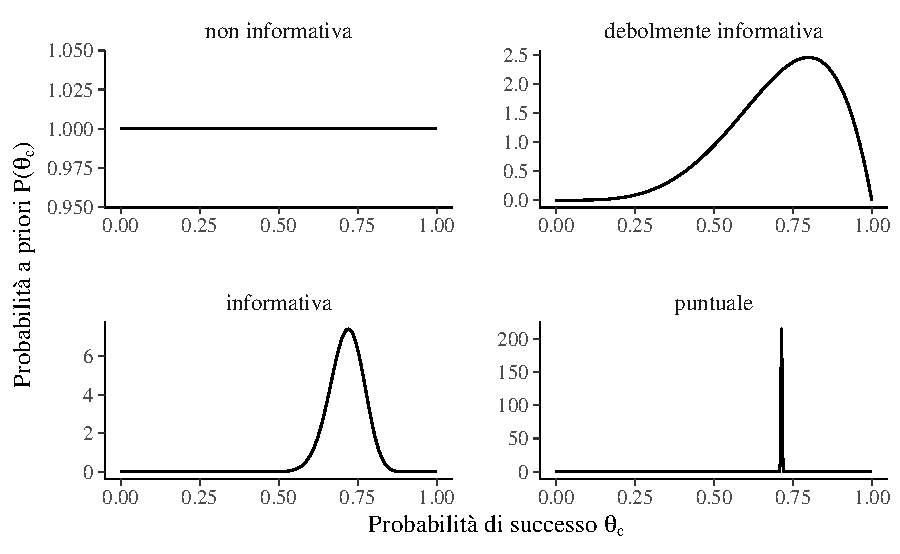
\includegraphics[width=0.8\linewidth]{025_intro_bayes_files/figure-latex/ch-03-02-models-types-of-priors-1} 

}

\caption{Esempi di distribuzioni a priori per il parametro $\theta_c$ nel Modello Binomiale.}\label{fig:ch-03-02-models-types-of-priors}
\end{figure}

\hypertarget{selezione-della-distribuzione-a-priori}{%
\subsection{Selezione della distribuzione a priori}\label{selezione-della-distribuzione-a-priori}}

La selezione delle distribuzioni a priori è stata spesso vista come una delle scelte più importanti che un ricercatore fa quando implementa un modello bayesiano in quanto può avere un impatto sostanziale sui risultati finali. La soggettività delle distribuzioni a priori è evidenziata dai critici come un potenziale svantaggio dei metodi bayesiani. A questa critica, \textcite{vandeSchoot2021modelling} rispondono dicendo che, al di là della scelta delle distribuzioni a priori, ci sono molti elementi del processo di inferenza statistica che sono soggettivi, ovvero la scelta del modello statistico e le ipotesi sulla distribuzione degli errori. In secondo luogo, \textcite{vandeSchoot2021modelling} notano come le distribuzioni a priori svolgono due importanti ruoli statistici: quello della ``regolarizzazione della stima'', ovvero, il processo che porta ad indebolire l'influenza indebita di osservazioni estreme, e quello del miglioramento dell'efficienza della stima, ovvero, la facilitazione dei processi di calcolo numerico di stima della distribuzione a posteriori. L'effetto della distribuzione a priori sulla distribuzione a posteriori verrà discusso nel Capitolo \ref{chapter-balance}.

\hypertarget{la-distribuzione-a-priori-per-i-dati-di-zetschefuture2019}{%
\subsection{\texorpdfstring{La distribuzione a priori per i dati di \textcite{zetschefuture2019}}{La distribuzione a priori per i dati di @zetschefuture2019}}\label{la-distribuzione-a-priori-per-i-dati-di-zetschefuture2019}}

In un problema concreto di analisi dei dati, la scelta della distribuzione a priori dipende dalle credenze a priori che vogliamo includere nell'analisi dei dati. Se non abbiamo alcuna informazione a priori, potremmo pensare di usare una distribuzione a priori uniforme, ovvero una Beta di parametri \(\alpha=1\) e \(\beta=1\). Questa, tuttavia, è una cattiva idea perché il risultato ottenuto non è invariante a seconda della trasformazione della scala dei dati (ad esempio, se esprimiamo l'altezza in cm piuttosto che in m). Il problema della \emph{riparametrizzazione} verrà discusso nel Capitolo ?? \textbf{TODO}. È invece raccomandato usare una distribuzione a priori poco informativa, come ad esempio \(\mbox{Beta}(2, 2)\).

Nella presente discussione, per fare un esempio, quale distribuzione a priori useremo una \(\mbox{Beta}(2, 10)\), ovvero:
\[
p(\theta) = \frac{\Gamma(12)}{\Gamma(2)\Gamma(10)}\theta^{2-1} (1-\theta)^{10-1}.
\]

\begin{Shaded}
\begin{Highlighting}[]
\NormalTok{bayesrules}\SpecialCharTok{::}\FunctionTok{plot\_beta}\NormalTok{(}\AttributeTok{alpha =} \DecValTok{2}\NormalTok{, }\AttributeTok{beta =} \DecValTok{10}\NormalTok{, }\AttributeTok{mean =} \ConstantTok{TRUE}\NormalTok{, }\AttributeTok{mode =} \ConstantTok{TRUE}\NormalTok{)}
\end{Highlighting}
\end{Shaded}

\begin{center}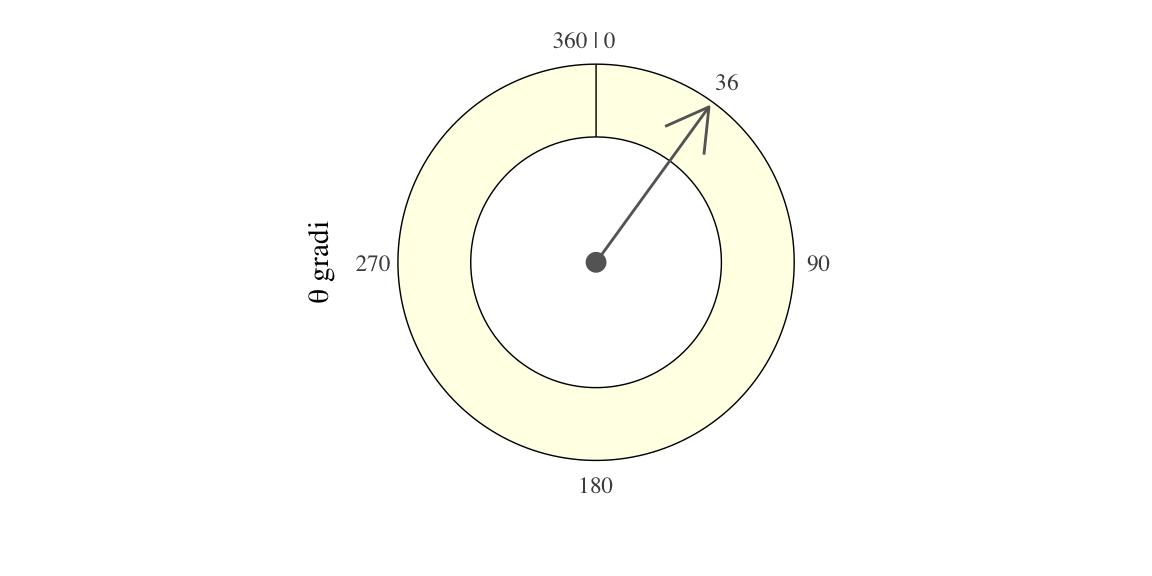
\includegraphics[width=0.8\linewidth]{025_intro_bayes_files/figure-latex/unnamed-chunk-1-1} \end{center}

\noindent
La \(\mbox{Beta}(2, 10)\) esprime la credenza che \(\theta\) assume valori \(< 0.5\), con il valore più plausibile pari a circa 0.1. Questo è assolutamente implausibile, nel caso dell'esempio in discussione. Adotteremo una tale distribuzione a priori solo per scopi didattici, per esplorare le conseguenze di tale scelta (molto più sensato sarebbe stato usare \(\mbox{Beta}(2, 2)\)).

\hypertarget{verosimiglianza}{%
\section{Verosimiglianza}\label{verosimiglianza}}

Oltre alla distribuzione a priori di \(\theta\), nel numeratore della regola di Bayes troviamo la funzione di verosimigliana. Iniziamo dunque con una definizione.

\begin{definition}
La \emph{funzione di verosimiglianza} \(\mathcal{L}(\theta \mid y) = f(y \mid \theta), \theta \in \Theta,\) è la funzione di massa o di densità di probabilità dei dati \(y\) vista come una funzione del parametro sconosciuto (o dei parametri sconosciuti) \(\theta\).
\end{definition}

Detto in altre parole, le funzioni di verosimiglianza e di (massa o densità di) probabilità sono formalmente identiche, ma è completamente diversa la loro interpretazione. Nel caso della funzione di massa o di densità di probabilità la distribuzione del vettore casuale delle osservazioni campionarie \(y\) dipende dai valori assunti dal parametro (o dai parametri) \(\theta\); nel caso della la funzione di verosimiglianza la credibilità assegnata a ciascun possibile valore \(\theta\) viene determinata avendo acquisita l'informazione campionaria \(y\) che rappresenta l'elemento condizionante. In altri termini, la funzione di verosimiglianza è lo strumento che consente di rispondere alla seguente domanda: avendo osservato i dati \(y\), quanto risultano (relativamente) credibili i diversi valori del parametro \(\theta\)?

Spesso per indicare la verosimiglianza si scrive \(\mathcal{L}(\theta)\) se è chiaro a quali valori \(y\) ci si riferisce. La verosimiglianza \(\mathcal{L}\) è una curva (in generale, una superficie) nello spazio \(\Theta\) del parametro (in generale, dei parametri) che riflette la credibilità relativa dei valori \(\theta\) alla luce dei dati osservati.

Notiamo un punto importante: la funzione \(\mathcal{L}(\theta \mid y)\) non è una funzione di densità. Infatti, essa non racchiude un'area unitaria.

In conclusione, la funzione di verosimiglianza descrive in termini relativi il sostegno empirico che \(\theta \in \Theta\) riceve da \(y\). Infatti, la funzione di verosimiglianza assume forme diverse al variare di \(y\) (lasciamo come esercizio da svolgere la verifica di questa affermazione).

\hypertarget{la-stima-di-massima-verosimiglianza}{%
\subsection{La stima di massima verosimiglianza}\label{la-stima-di-massima-verosimiglianza}}

La funzione di verosimiglianza rappresenta la ``credibilità relativa'' dei valori del parametro di interesse. Ma qual è il valore più credibile? Se utilizziamo soltanto la funzione di verosimiglianza, allora la risposta è data dalla stima di massima verosimiglinza.

\begin{definition}
Un valore di \(\theta\) che massimizza \(\mathcal{L}(\theta \mid y)\) sullo spazio parametrico \(\Theta\) è detto \emph{stima di massima verosimiglinza} (s.m.v.) di \(\theta\) ed è indicato con \(\hat{\theta}\):
\begin{equation}
\hat{\theta} = \argmax_{\theta \in \Theta} \mathcal{L}(\theta).
\end{equation}
\end{definition}

Il paradigma frequentista utilizza la funzione di verosimiglianza quale unico strumento per giungere alla stima del valore più credibile del parametro sconosciuto \(\theta\). Tale stima corrisponde al punto di massimo della funzione di verosimiglianza. In base all'approccio bayesiano, invece, il valore più credibile del parametro sconosciuto \(\theta\), anziché alla s.m.v., corrisponde invece alla moda (o media, o mediana) della distribuzione a posteriori \(p(\theta \mid y)\) che si ottiene combinando la verosimiglianza \(p(y \mid \theta)\) con la distribuzione a priori \(p(\theta)\). Per un approfondimento della stima di massima verosimiglianza si veda l'Appendice \ref{appendix:max-like}.

\hypertarget{la-log-verosimiglianza}{%
\subsection{La log-verosimiglianza}\label{la-log-verosimiglianza}}

Dal punto di vista pratico risulta più conveniente utilizzare, al posto della funzione di verosimiglianza, il suo logaritmo naturale, ovvero la funzione di log-verosimiglianza:
\begin{equation}
\ell(\theta) = \log \mathcal{L}(\theta).
\end{equation}
Poiché il logaritmo è una funzione strettamente crescente (usualmente si considera il logaritmo naturale), allora \(\mathcal{L}(\theta)\) e \(\ell(\theta)\) assumono il massimo (o i punti di massimo) in corrispondenza degli stessi valori di \(\theta\):
\[
\hat{\theta} = \argmax_{\theta \in \Theta} \ell(\theta) = \argmax_{\theta \in \Theta} \mathcal{L}(\theta).
\]
Per le proprietà del logaritmo, si ha
\begin{equation}
\ell(\theta) = \log \left( \prod_{i = 1}^n f(y \mid \theta) \right) = \sum_{i = 1}^n \log f(y \mid \theta).
\end{equation}

Si noti che non è necessario lavorare con i logaritmi, ma è fortemente consigliato. Il motivo è che i valori della verosimiglianza, in cui si moltiplicano valori di probabilità molto piccoli, possono diventare estremamente piccoli -- qualcosa come \(10^{-34}\). In tali circostanze, non è sorprendente che i programmi dei computer mostrino problemi di arrotondamento numerico. Le trasformazioni logaritmiche risolvono questo problema.

\begin{remark}
Seguendo una pratica comune, in questa dispensa useremo la notazione \(p(\cdot)\) per rappresentare quantità differenti, ovvero la funzione di verosimiglianza e la distribuzione a priori. Questo piccolo abuso di notazione riflette il seguente punto di vista: anche se la verosimiglianza non è una funzione di densità di probabilità, noi non vogliamo stressare questo aspetto, ma vogliamo piuttosto pensare alla verosimiglianza e alla distribuzione a priori come a due elementi che sono egualmente necessari per calcolare la distribuzione a posteriori. In altri termini, per così dire, questa notazione assegna lo stesso status epistemologico alle due diverse quantità che si trovano al numeratore della regola di Bayes.
\end{remark}

\begin{exercise}
Per i dati di \textcite{zetschefuture2019}, ovvero 23 ``successi'' in 30 prove, si trovi e si interpreti la funzione di verosimiglianza.
\end{exercise}

Per i dati di \textcite{zetschefuture2019} la funzione di verosimiglianza corrisponde alla funzione binomiale di parametro \(\theta \in [0, 1]\) sconosciuto. Abbiamo osservato un ``successo'' 23 volte in 30 ``prove'', dunque, \(y = 23\) e \(n = 30\). La funzione di verosimiglianza diventa
\begin{equation}
\mathcal{L}(\theta \mid y) = \frac{(23 + 7)!}{23!7!} \theta^{23} + (1-\theta)^7.
\label{eq:likebino23}
\end{equation}
Per costruire la funzione di verosimiglianza dobbiamo applicare la \eqref{eq:likebino23} tante volte, cambiando ogni volta il valore \(\theta\) ma \emph{tenendo sempre costante il valore dei dati}. Per esempio, se poniamo \(\theta = 0.1\)
\[
\mathcal{L}(\theta \mid y) = \frac{(23 + 7)!}{23!7!} 0.1^{23} + (1-0.1)^7
\]
\noindent
otteniamo

\begin{Shaded}
\begin{Highlighting}[]
\FunctionTok{dbinom}\NormalTok{(}\DecValTok{23}\NormalTok{, }\DecValTok{30}\NormalTok{, }\FloatTok{0.1}\NormalTok{)}
\CommentTok{\#\textgreater{} [1] 9.74e{-}18}
\end{Highlighting}
\end{Shaded}

\noindent
Se poniamo \(\theta = 0.2\)
\[
\mathcal{L}(\theta \mid y) = \frac{(23 + 7)!}{23!7!} 0.2^{23} + (1-0.2)^7
\]
\noindent
otteniamo

\begin{Shaded}
\begin{Highlighting}[]
\FunctionTok{dbinom}\NormalTok{(}\DecValTok{23}\NormalTok{, }\DecValTok{30}\NormalTok{, }\FloatTok{0.2}\NormalTok{)}
\CommentTok{\#\textgreater{} [1] 3.58e{-}11}
\end{Highlighting}
\end{Shaded}

\noindent
e così via. La figura \ref{fig:likefutexpect} --- costruita utilizzando 100 valori equispaziati \(\theta \in [0, 1]\) --- fornisce una rappresentazione grafica della funzione di verosimiglianza.

\begin{Shaded}
\begin{Highlighting}[]
\NormalTok{n }\OtherTok{\textless{}{-}} \DecValTok{30}
\NormalTok{y }\OtherTok{\textless{}{-}} \DecValTok{23}
\NormalTok{theta }\OtherTok{\textless{}{-}} \FunctionTok{seq}\NormalTok{(}\DecValTok{0}\NormalTok{, }\DecValTok{1}\NormalTok{, }\AttributeTok{length.out =} \DecValTok{100}\NormalTok{)}
\NormalTok{like }\OtherTok{\textless{}{-}} \FunctionTok{choose}\NormalTok{(n, y) }\SpecialCharTok{*}\NormalTok{ theta}\SpecialCharTok{\^{}}\NormalTok{y }\SpecialCharTok{*}\NormalTok{ (}\DecValTok{1} \SpecialCharTok{{-}}\NormalTok{ theta)}\SpecialCharTok{\^{}}\NormalTok{(n }\SpecialCharTok{{-}}\NormalTok{ y)}
\FunctionTok{tibble}\NormalTok{(theta, like) }\SpecialCharTok{\%\textgreater{}\%} 
  \FunctionTok{ggplot}\NormalTok{(}\FunctionTok{aes}\NormalTok{(}\AttributeTok{x =}\NormalTok{ theta, }\AttributeTok{y =}\NormalTok{ like)) }\SpecialCharTok{+}
  \FunctionTok{geom\_line}\NormalTok{() }\SpecialCharTok{+}
  \FunctionTok{labs}\NormalTok{(}
    \AttributeTok{y =} \FunctionTok{expression}\NormalTok{(}\FunctionTok{L}\NormalTok{(theta)),}
    \AttributeTok{x =} \FunctionTok{expression}\NormalTok{(}\StringTok{\textquotesingle{}Valori possibili di\textquotesingle{}} \SpecialCharTok{\textasciitilde{}}\NormalTok{ theta)}
\NormalTok{  )}
\end{Highlighting}
\end{Shaded}

\begin{figure}[h]

{\centering 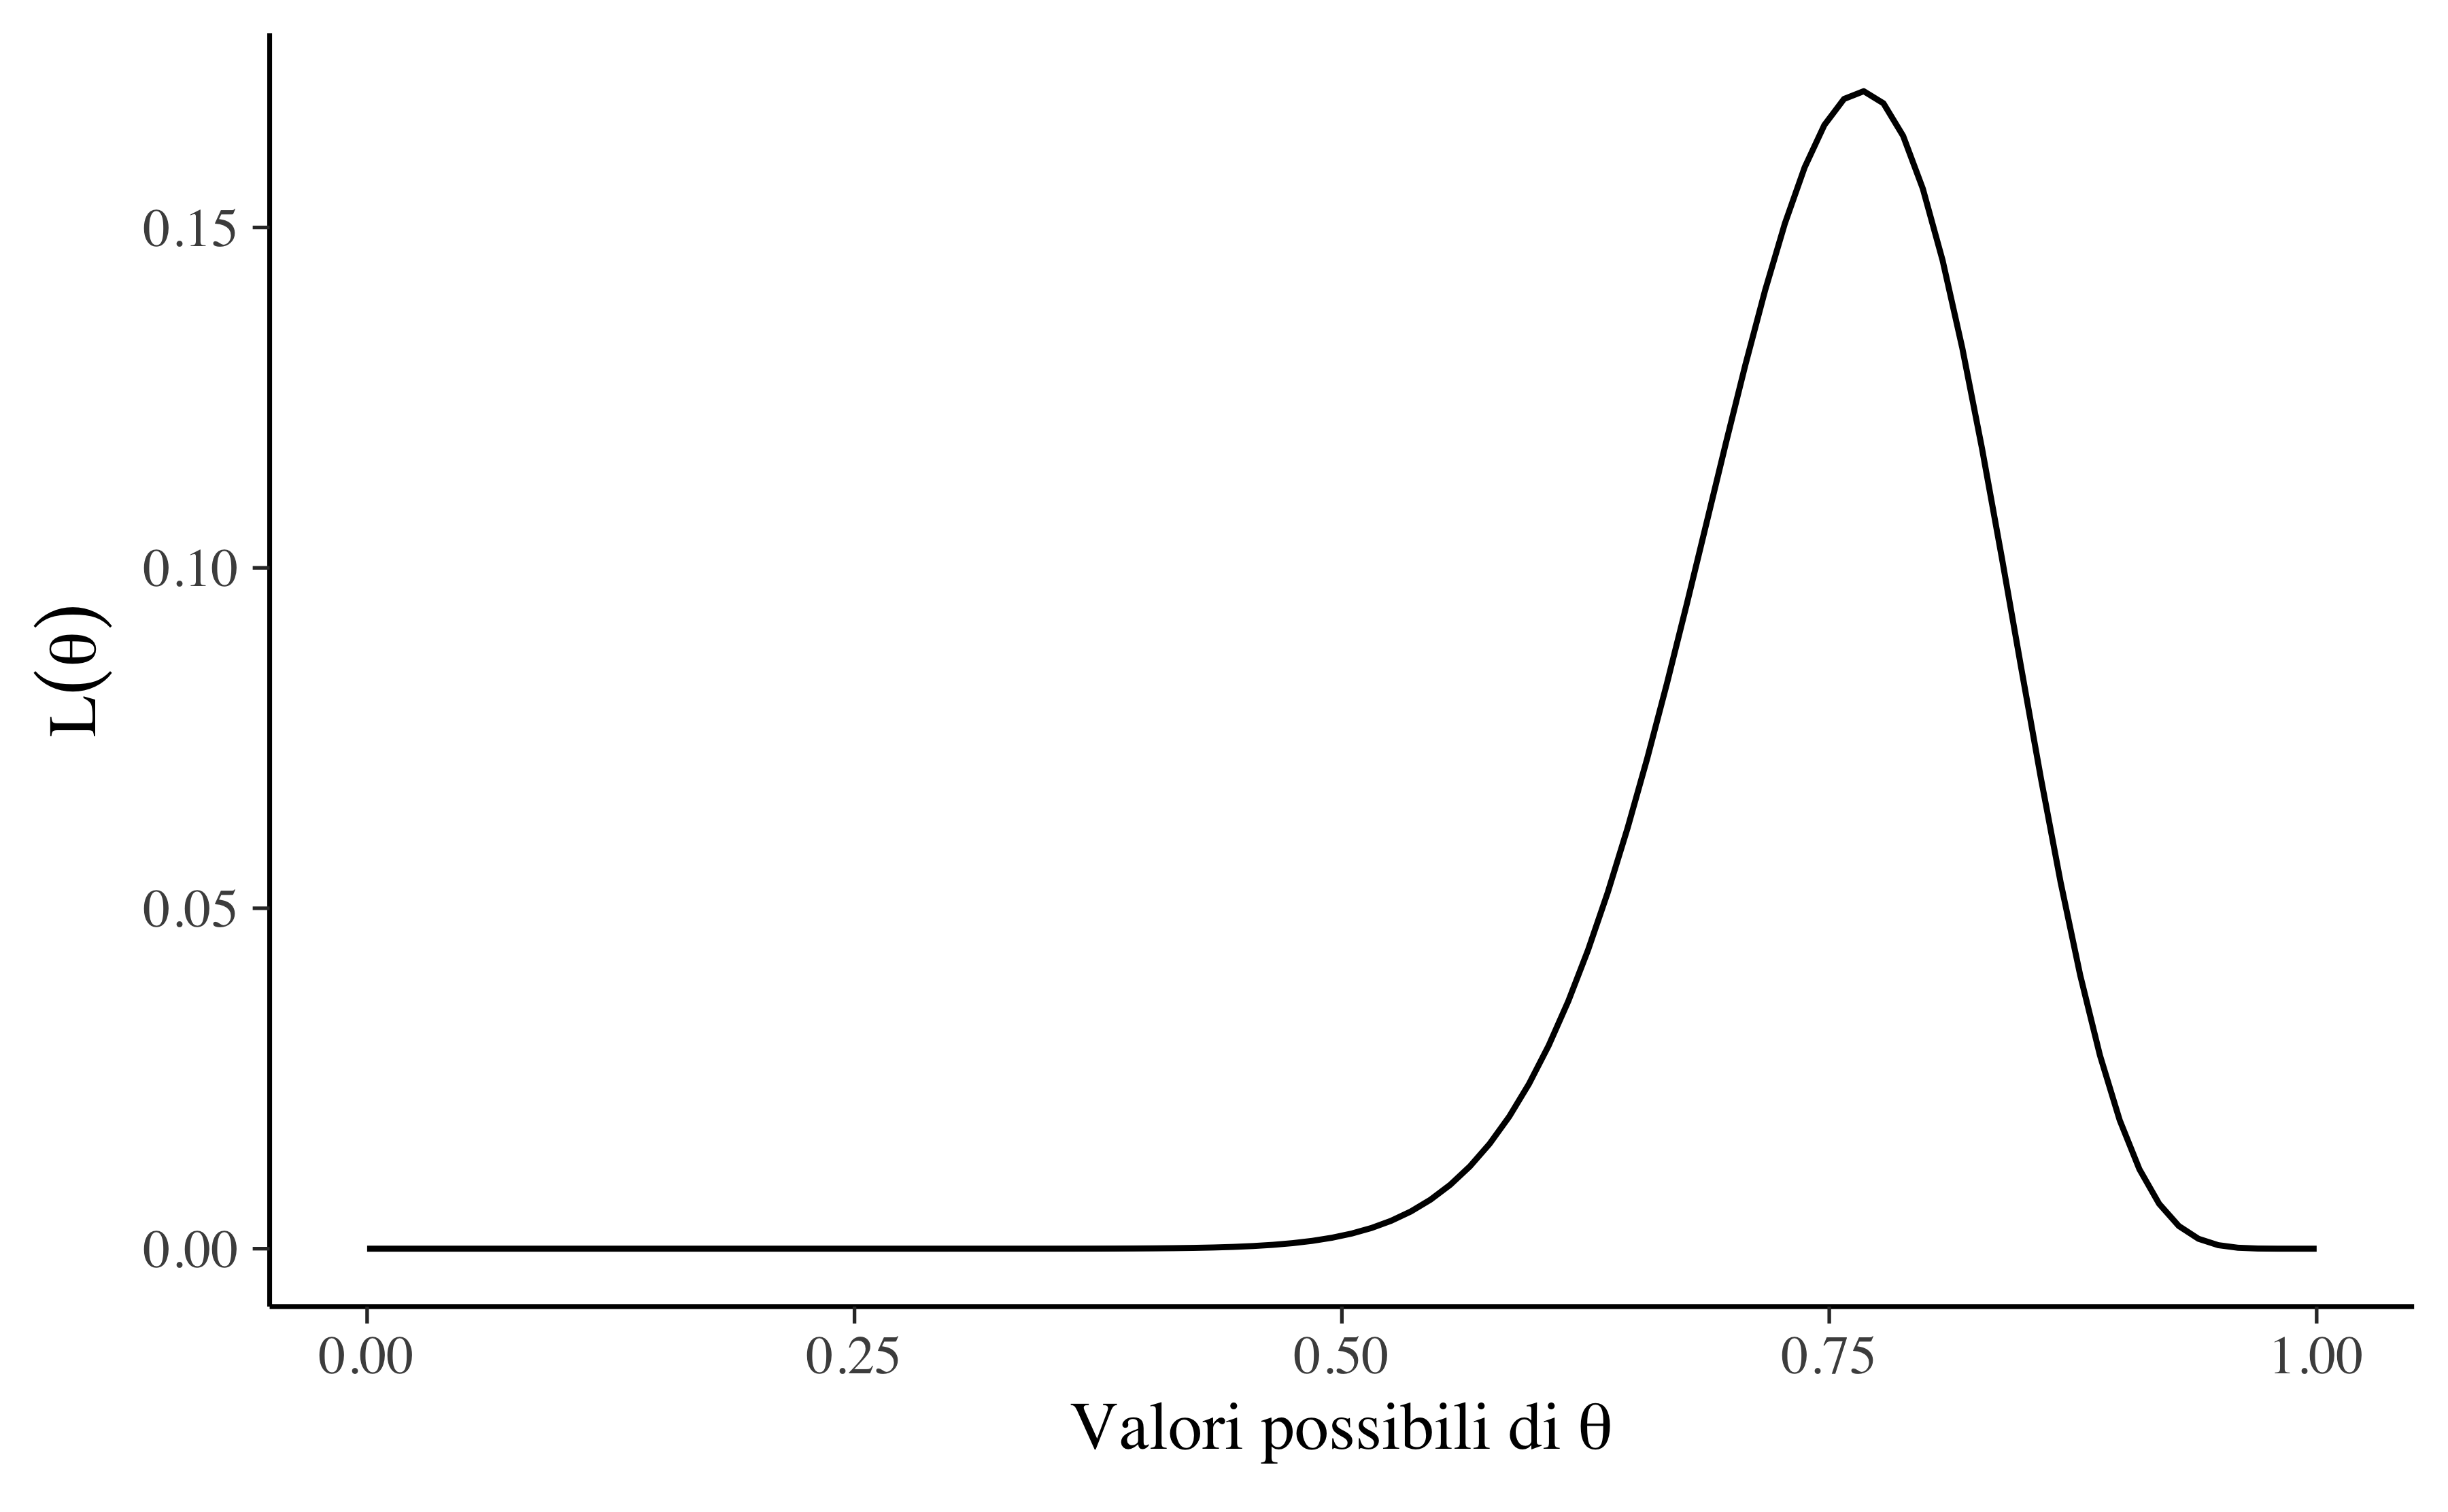
\includegraphics[width=0.8\linewidth]{025_intro_bayes_files/figure-latex/likefutexpect-1} 

}

\caption{Funzione di verosimiglianza nel caso di 23 successi in 30 prove.}\label{fig:likefutexpect}
\end{figure}

Come possiamo interpretare la curva che abbiamo ottenuto? Per alcuni valori \(\theta\) la funzione di verosimiglianza assume valori piccoli; per altri valori \(\theta\) la funzione di verosimiglianza assume valori più grandi. Questi ultimi sono i valori di \(\theta\) ``più credibili'' e il valore 23/30 è il valore più credibile di tutti. La funzione di verosimiglianza di \(\theta\) valuta la compatibilità dei dati osservati \(Y = y\) con i diversi possibili valori \(\theta\). In termini più formali possiamo dire che la funzione di verosimiglianza ha la seguente interpretazione: sulla base dei dati, \(\theta_1 \in \Theta\) è più credibile di \(\theta_2 \in \Theta\) come indice del modello probabilistico generatore delle osservazioni se \(\mathcal{L}(\theta_1) > \mathcal{L}(\theta_1)\).

\hypertarget{sec:const-normaliz-bino23}{%
\section{La verosimiglianza marginale}\label{sec:const-normaliz-bino23}}

Per il calcolo di \(p(\theta \mid y)\) è necessario dividere il prodotto tra la distribuzione a priori e la verosimiglianza per una costante di normalizzazione. Tale costante di normalizzazione, detta \emph{verosimiglianza marginale}, ha lo scopo di fare in modo che \(p(\theta \mid y)\) abbia area unitaria.

Si noti che il denominatore della regola di Bayes (ovvero la verosimiglianza marginale) è sempre espresso nei termini di un integrale. Tranne in pochi casi particolari, tale integrale non ha una soluzione analitica. Per questa ragione, l'inferenza bayesiana procede calcolando una approssimazione della distribuzione a posteriori mediante metodi numerici.

\begin{exercise}
Si trovi la verosimiglianza maginale per i dati di \textcite{zetschefuture2019}.

Supponiamo che nel numeratore bayesiano la verosimiglianza sia moltiplicata per una distribuzione uniforme, \(\mbox{Beta}(1, 1)\). In questo caso, il prodotto si riduce alla funzione di verosimiglianza. In riferimento ai dati di \textcite{zetschefuture2019}, la costante di normalizzazione per si ottiene semplicemente marginalizzando la funzione di verosimiglianza \(p(y = 23, n = 30 \mid \theta)\) sopra \(\theta\), ovvero risolvendo l'integrale:
\begin{equation}
p(y = 23, n = 30) = \int_0^1 \binom{30}{23} \theta^{23} (1-\theta)^{7} \,\operatorname {d}\!\theta.
\label{eq:intlikebino23}
\end{equation}
\noindent
Una soluzione numerica si trova facilmente usando \(\R\):

\begin{Shaded}
\begin{Highlighting}[]
\NormalTok{like\_bin }\OtherTok{\textless{}{-}} \ControlFlowTok{function}\NormalTok{(theta) \{}
  \FunctionTok{choose}\NormalTok{(}\DecValTok{30}\NormalTok{, }\DecValTok{23}\NormalTok{) }\SpecialCharTok{*}\NormalTok{ theta}\SpecialCharTok{\^{}}\DecValTok{23} \SpecialCharTok{*}\NormalTok{ (}\DecValTok{1} \SpecialCharTok{{-}}\NormalTok{ theta)}\SpecialCharTok{\^{}}\DecValTok{7}
\NormalTok{\}}
\FunctionTok{integrate}\NormalTok{(like\_bin, }\AttributeTok{lower =} \DecValTok{0}\NormalTok{, }\AttributeTok{upper =} \DecValTok{1}\NormalTok{)}\SpecialCharTok{$}\NormalTok{value}
\CommentTok{\#\textgreater{} [1] 0.0323}
\end{Highlighting}
\end{Shaded}

\noindent
La derivazione analitica della costante di normalizzazione qui discussa è fornita nell'Appendice \ref{appendix:const-norm-bino23}.
\end{exercise}

\hypertarget{distribuzione-a-posteriori}{%
\section{Distribuzione a posteriori}\label{distribuzione-a-posteriori}}

La distribuzione a postreriori si trova applicando il teorema di Bayes:
\[
\text{probabilità a posteriori} = \frac{\text{probabilità a priori} \cdot \text{verosimiglianza}}{\text{costante di normalizzazione}}
\]
Ci sono due metodi principali per calcolare la distribuzione a posteriori \(p(\theta \mid y)\):

\begin{itemize}
\item
  una precisa derivazione matematica formulata nei termini della distribuzione a priori coniugata alla distribuzione a posteriori (si veda il Capitolo \ref{chapter-distr-coniugate}); tale procedura però ha un'applicabilità molto limitata;
\item
  un metodo approssimato, molto facile da utilizzare in pratica, che dipende da metodi Monte Carlo basati su Catena di Markov (MCMC); questo problema verrà discusso nel Capitolo ??
\end{itemize}

\hypertarget{considerazioni-conclusive}{%
\section*{Considerazioni conclusive}\label{considerazioni-conclusive}}
\addcontentsline{toc}{section}{Considerazioni conclusive}

Questo Capitolo ha brevemente passato in rassegna alcuni concetti di base dell'inferenza statistica bayesiana. In base all'approccio bayesiano, invece di dire che il parametro di interesse di un modello statistico ha un valore vero ma sconosciuto, diciamo che, prima di eseguire l'esperimento, è possibile assegnare una distribuzione di probabilità, che chiamano stato di credenza, a quello che è il vero valore del parametro. Questa distribuzione a priori può essere nota (per esempio, sappiamo che la distribuzione dei punteggi del QI è normale con media 100 e deviazione standard 15) o può essere del tutto arbitraria. L'inferenza bayesiana procede poi nel modo seguente: si raccolgono alcuni dati e si calcola la probabilità dei possibili valori del parametro alla luce dei dati osservati e delle credenze a priori. Questa nuova distribuzione di probabilità è chiamata ``distribuzione a posteriori'' e riassume l'incertezza dell'inferenza. I concetti importanti che abbiamo appreso in questo Capitolo sono quelli di distribuzione a priori, verosimiglianza, verosimiglianza marginale e distribuzione a posteriori. Questi sono i concetti fondamentali della statistica bayesiana.


% Bibliography
%%%%%%%%%%%%%%%%%%%%%%%%%%%%%%%%%%%%%%%%%%%%%%%%%%%%%%%%%%

\backmatter
\SmallMargins

\printbibliography
\onecolumn


% Tables (of tables, of figures)
%%%%%%%%%%%%%%%%%%%%%%%%%%%%%%%%%%%%%%%%%%%%%%%%%%%%%%%%%%


\cleardoublepage
\LargeMargins
\listoffigures


% After-body (LaTeX code inclusion)
%%%%%%%%%%%%%%%%%%%%%%%%%%%%%%%%%%%%%%%%%%%%%%%%%%%%%%%%%%




% Back cover
%%%%%%%%%%%%%%%%%%%%%%%%%%%%%%%%%%%%%%%%%%%%%%%%%%%%%%%%%%%

% Even page, small margins, no running head, no page number.
\evenpage
\SmallMargins
\thispagestyle{empty}

\begin{normalsize}

\begin{description}

\selectlanguage{italian}
\item[Abstract]
This document contains the material of the lessons of Psicometria B000286 (2021/2022) aimed at students of the first year of the Degree Course in Psychological Sciences and Techniques of the University of Florence, Italy.
\item[Keywords]
Data science, Bayesian statistics.
~\\

\end{description}

\end{normalsize}


\end{document}
